\scanpage{52}
% archive sheet number: 51
\diagram{\begin{tikzcd}[ampersand replacement=\&]
\unsure{O|\mathcal O}\&\widehat O_{q_1}\arrow[l]\arrow[d]\&O_{q_1}\arrow[l]\arrow[d]\\
\&\widehat O_{q_1,q_0}\&O_{q_0}\arrow[l]
\end{tikzcd}}
\[\otimes\]

\figure{\begin{tikzpicture}
\draw (-.7,.35)--(-.45,.8);\fill (-.7,.1) circle (.04);\node[below] at (-.7,.05) {$x$};
\draw (-.25,1.0)..controls (-.05,.3) and (.2,.15)..(.55,-.05);\fill (-.05,.48) circle (.035);
\draw (.05,.95)--(.65,.8);\fill (.85,.86) circle (.035);\fill (1.08,.8) circle (.035);
\draw[line width=1.2pt] (3.3,-.7)--(5,-.7);\foreach \x in {3.3,4.2,5}{\fill (\x,-.7) circle (.065);}
\end{tikzpicture}}

$x$, $\unsure{p|q}$ \unsure{fixés|finis}
\figure{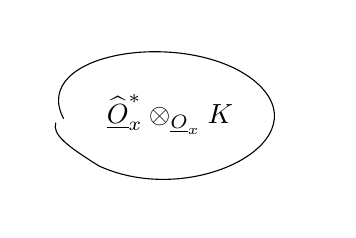
\begin{tikzpicture}
\node at (0,0) {$\widehat{\underline O}_x^{\unsure{*}}\otimes_{\underline O_x}K$};
\draw (-1.35,-.05)..controls (-1.8,.8) and (.2,1.1)..(1.05,.45)..controls (2,-.3) and (.3,-1.2)..(-.9,-.65)..controls (-1.3,-.4) and (-1.5,-.25)..(-1.45,-.1);
\end{tikzpicture}}

\[ A_{[p\supset q]} \]
\diagram{\begin{tikzcd}[ampersand replacement=\&]
A_{[p]}=\widehat A_p\&\\
A_p\arrow[u]\arrow[r]\&A_q/q^n A_q
\end{tikzcd}}
\diagram{\begin{tikzcd}[ampersand replacement=\&]
A_{[p]}=\widehat A_p\&A_p\arrow[l]
\end{tikzcd}}

\[
\begin{aligned}
A_{[p,q]}&=\varprojlim_n\underbrace{A_{[p]}\otimes_A A_q/q^n A_q}\\
&\hspace{3cm}\Vert\\
&\hspace{1cm} A_{[p]}\otimes_{A_p}A_q/q^n A_q\\
&\hspace{3cm}\Vert\\
&\hspace{1cm} A_{[p]}/q^n A_{[p]}\otimes_{\deleted{\unsure{A_q}}A_p} A_q/q^n A_q\\
&\hspace{3cm}\Vert\\
&\hspace{1cm}\deleted{\unsure{(A/q^n A}}\\
&\hspace{1cm} A_{[p]}/q^n A_{[p]}\otimes_{A_p} A_q\\
&\hspace{3cm}\Vert\\
&\hspace{1cm}\underbrace{A_{[p]}/q^n A_{[p]}}\otimes_A A_q\\
&\hspace{3cm}\Vert\\
&\hspace{1cm}\deleted{\unsure{A_p}(A/q^n A)_{[p]}}
\end{aligned}
\]
\margin{On peut y \unsure{remplacer} $q^n$ par $q^{(n)}$}
\margin{\unsure{anneau} \unsure{semi local}, \unsure{non complet}, \unsure{mais quotient} \unsure{d'un complété} \unsure{localisé} de $\widehat{A_p/q A_p}\otimes_{A_p/q A_p}\unsure{L|1}$}
\diagram{\begin{tikzcd}[ampersand replacement=\&]
\widehat{A_p/q^n A_p}=(A/q^n A)_{[p]}\&{}\arrow[l]
\end{tikzcd}}

\figure{\begin{tikzpicture}[scale=.5]
\draw (0,4.6) to[out=-80,in=10] (-2.4,2.5) to[out=190,in=70] (-2.8,1.6) to[out=250,in=20] (-4.2,.4) to[out=200,in=60] (-5,-.6);
\draw (6.5,5) to[out=-65,in=65] (7,-.8);
\end{tikzpicture}}
